\subsection{Diffraction}
\initial{D}iffraction has to do with how waves soread and interact after whay have passed through one ore several onenings.
The openings can be some distance appart, or close together and form some sort of grid.
If there is only one opening the waves will "bend" aftet they have passed the opening and create half-circles.
With two openings the two bent waves will interact with each other and form what we call an interference pattern.
This pattern is made because the waves amplify and nullify each other at different points.
If the waves has passed through a grid the pattern becomes even more spectular.

Many different kinds of grid can give rise to diffraction and interference patterns.
Even the atomic structure in solid matter!
In solid matter, mainly crystals, the atomic structure repeates itself over and over again, and makes planes that can be seen as openings in a grid.

The reason diffraction is such an important and powerful technique is that different grids gives rise to distinct patterns.
How far away the openings in the grid is spaced form each other determines how the pattern will look.
This is also true for the patterns made by crystals.
In other words, the diffraction pattern of a solid matter is like its finger print.

\begin{center}
	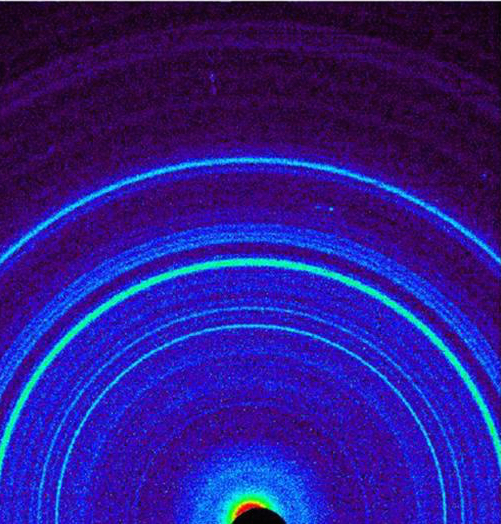
\includegraphics[width=0.45\textwidth]{Curiosity_diffraction.jpg}
\end{center}

Waves used in diffraction is usually light, or electromagnetic waves, though this is not necessarily the case.
All kinds of waves form diffraction patterns.
The waves in water, sound waves, waves in light and "waves" made by small particles like electrons and protons.
That is the second reason diffraction is such a powerful tool for scientists.
On Curiosity mostly X-rays are used.